\documentclass[conference]{IEEEtran}
\IEEEoverridecommandlockouts
\usepackage{cite}
\usepackage{amsmath,amssymb,amsfonts}
\usepackage{graphicx}
\usepackage{textcomp}
\usepackage{xcolor}
\usepackage{booktabs}
\usepackage[utf8]{inputenc}
\usepackage[vietnamese]{babel}
\def\BibTeX{{\rm B\kern-.05em{\sc i\kern-.025em b}\kern-.08em
    T\kern-.1667em\lower.7ex\hbox{E}\kern-.125emX}}

\begin{document}

\title{Xây dựng hệ thống tạo mô hình 3D từ ảnh và mô tả văn bản (AI đa phương thức).}

\author{
\IEEEauthorblockN{Nguyễn Hoàng Anh}
\IEEEauthorblockA{\textit{Lớp KHMT 17-01} \\
\textit{Trường Đại học Đại Nam}\\
Hà Nội, Việt Nam}
}

\maketitle

\begin{abstract}
Báo cáo này trình bày một hệ thống học sâu đa phương thức có khả năng sinh ra đám mây điểm 3D có màu sắc từ một ảnh 2D và một mô tả văn bản ngắn. Mô hình kết hợp bộ mã hóa OpenCLIP ViT-B/32 (cố định trọng số) với bộ giải mã dạng Transformer theo chiến lược thô-đến-tinh để tạo ra đám mây điểm dày đặc gồm 2.048 điểm. Mô hình được huấn luyện trên tập dữ liệu Cap3D ABO gồm 11.464 đối tượng trong 15 epoch trên GPU NVIDIA Tesla T4 và đạt Chamfer Distance 0,0045 cùng F-Score@0.01 là 0,9592 trên tập kiểm tra. Ngoài ra, một module dịch tự động tiếng Việt sang tiếng Anh được tích hợp vào pipeline suy luận nhằm cải thiện kết quả khi người dùng nhập mô tả bằng tiếng Việt.
\end{abstract}

\begin{IEEEkeywords}
sinh đám mây điểm 3D, học đa phương thức, CLIP, transformer decoder, Chamfer Distance
\end{IEEEkeywords}

% ─────────────────────────────────────────────
\section{Giới Thiệu}

Tái tạo hình học 3D từ quan sát 2D là một bài toán trọng tâm trong thị giác máy tính, với ứng dụng trong robot học, thực tế tăng cường và tạo nội dung số. Các mô hình ngôn ngữ-thị giác lớn như CLIP \cite{clip} mở ra hướng mới: điều kiện hóa việc sinh 3D đồng thời trên cả ảnh \emph{lẫn} mô tả ngôn ngữ tự nhiên. Điều kiện hóa đa phương thức này giúp mô hình tận dụng cả ngoại hình trực quan lẫn ngữ nghĩa, từ đó cải thiện chất lượng tái tạo.

Trong đồ án này, chúng tôi thiết kế và huấn luyện một pipeline đầu-cuối nhận một ảnh render đơn và một câu mô tả văn bản làm đầu vào, và xuất ra đám mây điểm 3D có màu dày đặc. Mô hình được đánh giá trên chuẩn Cap3D ABO \cite{cap3d} và cho thấy độ chính xác tái tạo tốt chỉ sau 15 epoch huấn luyện trên một GPU T4.

% ─────────────────────────────────────────────
\section{Phương Pháp}

\subsection{Kiến Trúc Tổng Quan}

Hình~\ref{fig:arch} minh họa tổng quan pipeline. Pipeline gồm ba thành phần chính:

\begin{figure}[htbp]
\centerline{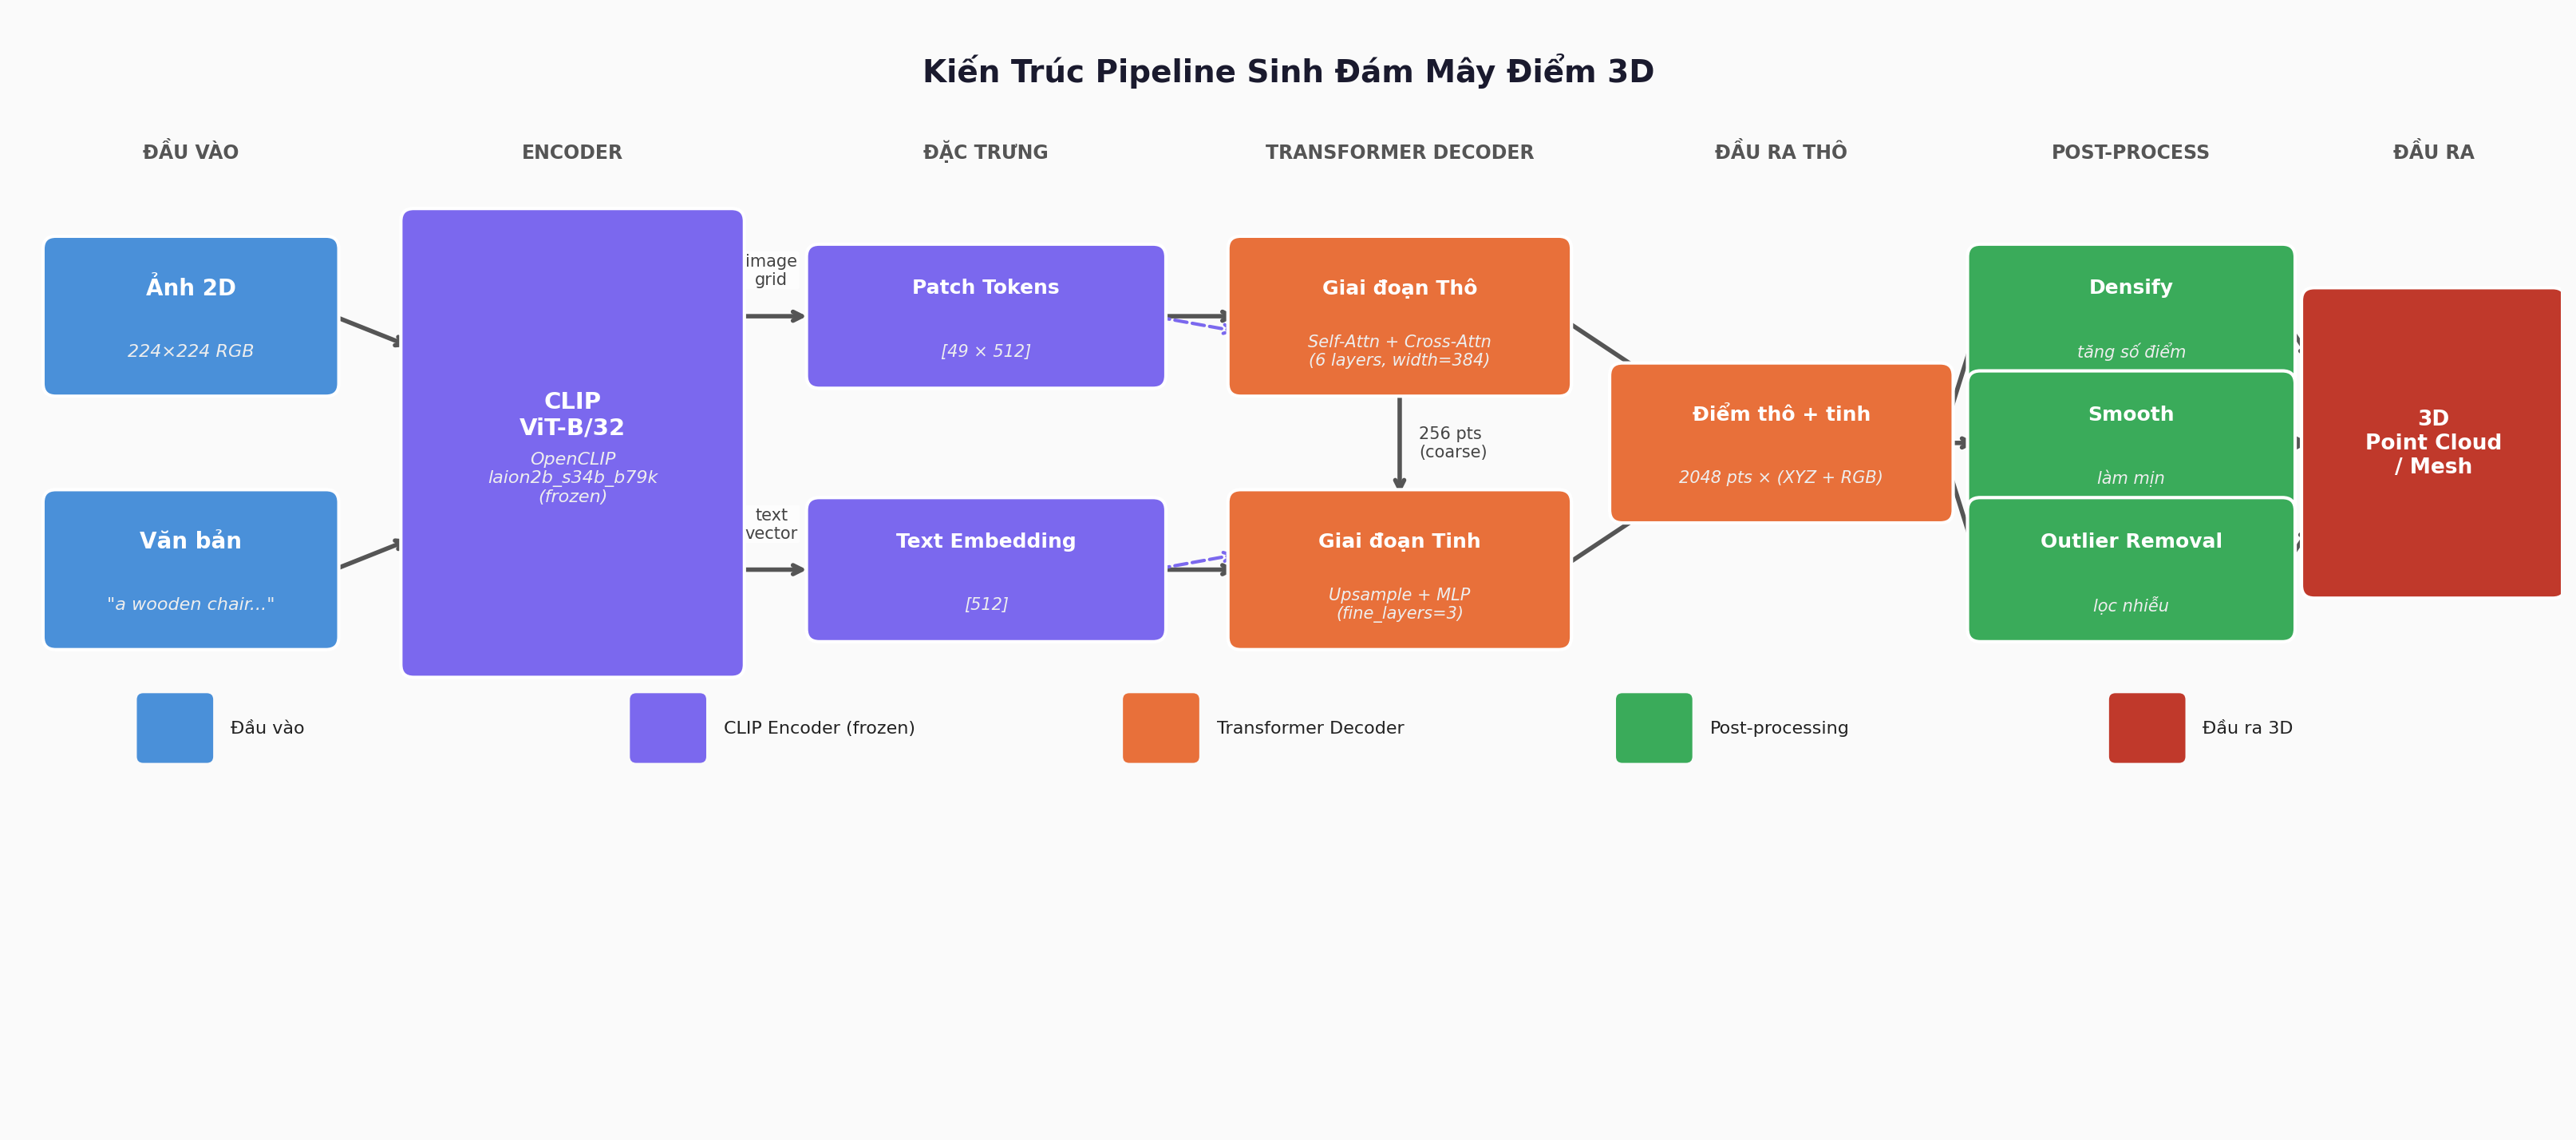
\includegraphics[width=\linewidth]{image_report/fig_architecture.png}}
\caption{Kiến trúc pipeline sinh đám mây điểm 3D đa phương thức.}
\label{fig:arch}
\end{figure}

\begin{itemize}
    \item \textbf{Bộ mã hóa ảnh.} Mô hình OpenCLIP ViT-B/32 \cite{clip} được giữ cố định (frozen) và trích xuất đặc trưng không gian từ ảnh đầu vào. Thay vì chỉ dùng token CLS, chúng tôi trích xuất toàn bộ $49$ patch token từ lớp transformer cuối cùng, tạo ra biểu diễn không gian phong phú với kích thước $[49, 512]$.

    \item \textbf{Bộ mã hóa văn bản.} Cùng mô hình CLIP mã hóa câu mô tả thành vector 512 chiều. Tại thời điểm suy luận, đầu vào tiếng Việt được tự động dịch sang tiếng Anh bằng MarianMT \texttt{opus-mt-vi-en} \cite{marian} trước khi mã hóa, vì mô hình được huấn luyện với caption tiếng Anh.

    \item \textbf{Bộ giải mã Transformer.} Bộ giải mã thô-đến-tinh với các query token có thể học được sinh ra đám mây điểm 3D theo hai giai đoạn. Giai đoạn thô tạo 256 điểm hạt giống qua self-attention trên các query và cross-attention đến patch feature của ảnh, có điều kiện trên embedding văn bản. Giai đoạn tinh nâng mẫu lên 2.048 điểm và dự đoán màu RGB cho từng điểm.
\end{itemize}

Tổng số tham số có thể huấn luyện là 21,3 triệu (trong tổng 172,6 triệu tham số, với CLIP được cố định).

\subsection{Hậu Xử Lý Đám Mây Điểm}

Đám mây điểm thô từ decoder được qua ba bước hậu xử lý trước khi hiển thị:
\begin{itemize}
    \item \textbf{Densify (tăng dày).} Bổ sung thêm điểm bằng cách nội suy giữa các điểm lân cận, giúp bề mặt đầy hơn khi render.
    \item \textbf{Smooth (làm mịn).} Di chuyển mỗi điểm về phía trung bình của $k$ điểm lân cận gần nhất, giảm nhiễu cục bộ.
    \item \textbf{Outlier Removal (lọc ngoại lệ).} Loại bỏ các điểm cách xa hơn $2\sigma$ so với tâm của đám mây, giúp loại bỏ điểm nhiễu xa.
\end{itemize}
Sau đó đám mây điểm được tái tạo thành mesh 3D bằng thuật toán Poisson Surface Reconstruction qua thư viện Open3D.

\subsection{Hàm Mất Mát}

Mô hình được huấn luyện với tổ hợp có trọng số của nhiều hàm mất mát:
\begin{equation}
    \mathcal{L} = \lambda_{cd}\,\mathcal{L}_{CD} + \lambda_{color}\,\mathcal{L}_{color} + \lambda_{rep}\,\mathcal{L}_{rep} + \lambda_{uni}\,\mathcal{L}_{uni} + \lambda_{n}\,\mathcal{L}_{normal}
\end{equation}
trong đó $\mathcal{L}_{CD}$ là Chamfer Distance hai chiều, $\mathcal{L}_{color}$ là mất mát màu sắc L2, các số hạng còn lại thúc đẩy tính đẩy nhau giữa các điểm, độ đồng đều và độ mượt bề mặt. Trọng số được đặt là $\lambda_{cd}{=}1{,}0$, $\lambda_{color}{=}0{,}5$, $\lambda_{rep}{=}0{,}1$, $\lambda_{uni}{=}0{,}05$, $\lambda_{n}{=}0{,}05$.

% ─────────────────────────────────────────────
\section{Dữ Liệu}

Dự án sử dụng tập con \textbf{Cap3D ABO} \cite{cap3d}, bao gồm các đối tượng Amazon Berkeley Objects (ABO) với ảnh render và đám mây điểm ground-truth tương ứng. Sau khi lọc các đối tượng có đầy đủ cả file đám mây điểm (.ply hoặc .pt) \emph{và} ít nhất một ảnh render, chúng tôi thu được 14.290 đối tượng hợp lệ.

Tập dữ liệu được chia theo tỉ lệ 80/10/10 bằng seed ngẫu nhiên cố định, thu được lần lượt 11.464 / 1.433 / 1.433 đối tượng cho huấn luyện, kiểm định và kiểm tra. Mỗi đối tượng được biểu diễn bởi một ảnh RGB kích thước $224{\times}224$ và một caption tiếng Anh từ Cap3D. Đám mây điểm ground-truth được lấy mẫu xuống 2.048 điểm với tọa độ XYZ và màu RGB.

Hình~\ref{fig:dataset} minh họa một số mẫu ảnh render từ tập dữ liệu ABO, bao gồm nhiều loại đồ vật gia dụng như ghế, bàn, tủ và đồ dùng văn phòng.

\begin{figure}[htbp]
\centerline{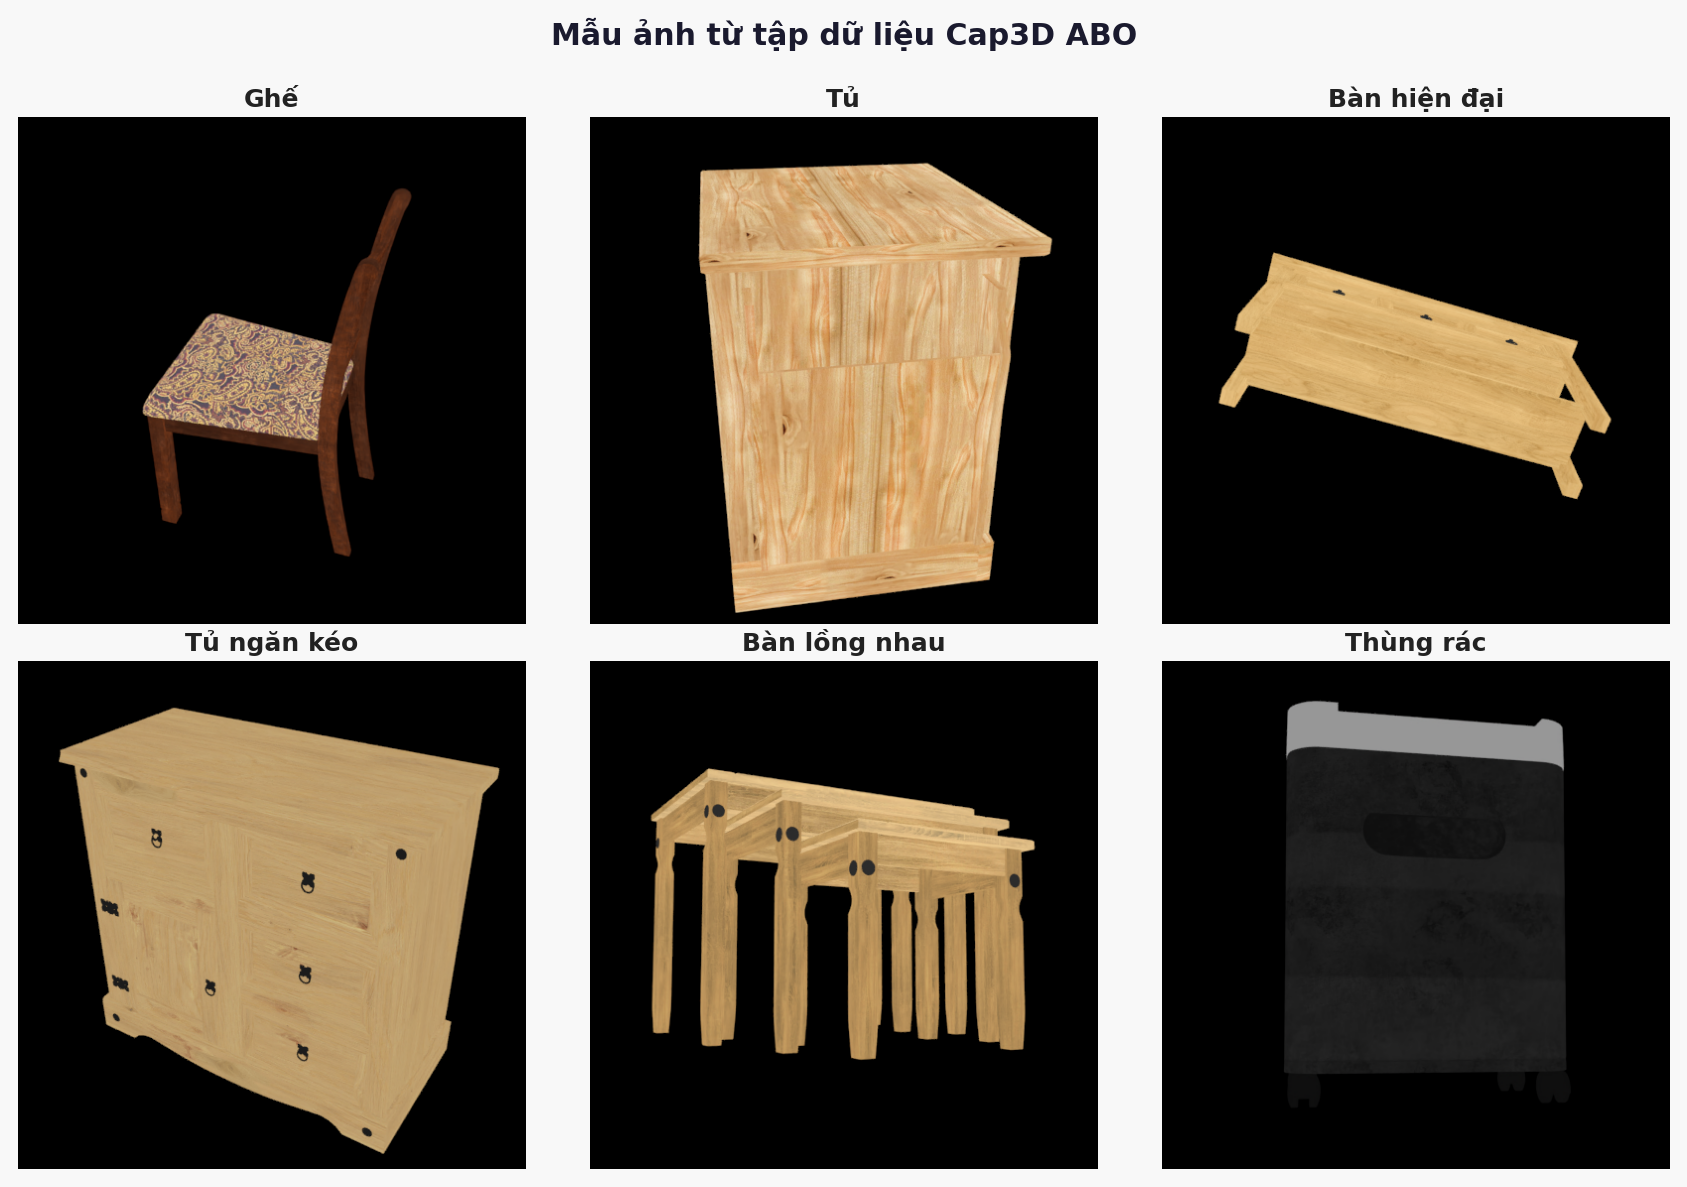
\includegraphics[width=\linewidth]{image_report/fig_dataset_samples.png}}
\caption{Mẫu ảnh render từ tập dữ liệu Cap3D ABO (Amazon Berkeley Objects).}
\label{fig:dataset}
\end{figure}

% ─────────────────────────────────────────────
\section{Chi Tiết Huấn Luyện}

Quá trình huấn luyện được thực hiện trên Google Colab với GPU \textbf{NVIDIA Tesla T4} (14,56\,GB VRAM). Mixed-precision training (AMP, forward pass float16, trọng số float32) được sử dụng để fit batch size 64 trong bộ nhớ GPU. Bộ tối ưu là AdamW với learning rate $10^{-3}$, weight decay $0{,}01$ và cosine annealing với 5 epoch warm-up. Early stopping patience được đặt là 25 epoch, tối đa 100 epoch. Mỗi epoch mất khoảng 2 giờ 14 phút. Quá trình huấn luyện dừng sau 15 epoch (tổng $\approx$33 giờ).

% ─────────────────────────────────────────────
\section{Kết Quả}

\subsection{Đánh Giá Định Lượng}

Bảng~\ref{tab:results} trình bày Chamfer Distance (CD, càng thấp càng tốt) và F-Score@0.01 (càng cao càng tốt) trên tập kiểm tra, sử dụng checkpoint tốt nhất trên tập kiểm định (epoch 14).

\begin{table}[htbp]
\caption{Kết Quả Định Lượng trên Tập Kiểm Tra Cap3D ABO}
\begin{center}
\begin{tabular}{lcc}
\toprule
\textbf{Độ đo} & \textbf{Kiểm định} & \textbf{Kiểm tra} \\
\midrule
Chamfer Distance (CD) $\downarrow$ & 0,0044 & 0,0045 \\
F-Score @ 0.01 $\uparrow$          & ---    & 0,9592 \\
\midrule
Epoch tốt nhất        & \multicolumn{2}{c}{14} \\
Tổng epoch đã huấn luyện & \multicolumn{2}{c}{15} \\
\bottomrule
\end{tabular}
\label{tab:results}
\end{center}
\end{table}

CD trên tập kiểm định và kiểm tra gần như bằng nhau (0,0044 so với 0,0045) cùng F-Score cao 0,9592 cho thấy mô hình có khả năng tổng quát hóa tốt mà không bị overfit.

\subsection{Đánh Giá Định Tính}

Hình~\ref{fig:result_en} và Hình~\ref{fig:result_vi} minh họa đám mây điểm 3D đầu ra cho cùng một ảnh ghế, lần lượt với caption tiếng Anh và caption tiếng Việt (được dịch tự động). Cả hai đầu vào cho kết quả tương đương nhau, chứng tỏ hiệu quả của module dịch tự động.

\begin{figure}[htbp]
\centerline{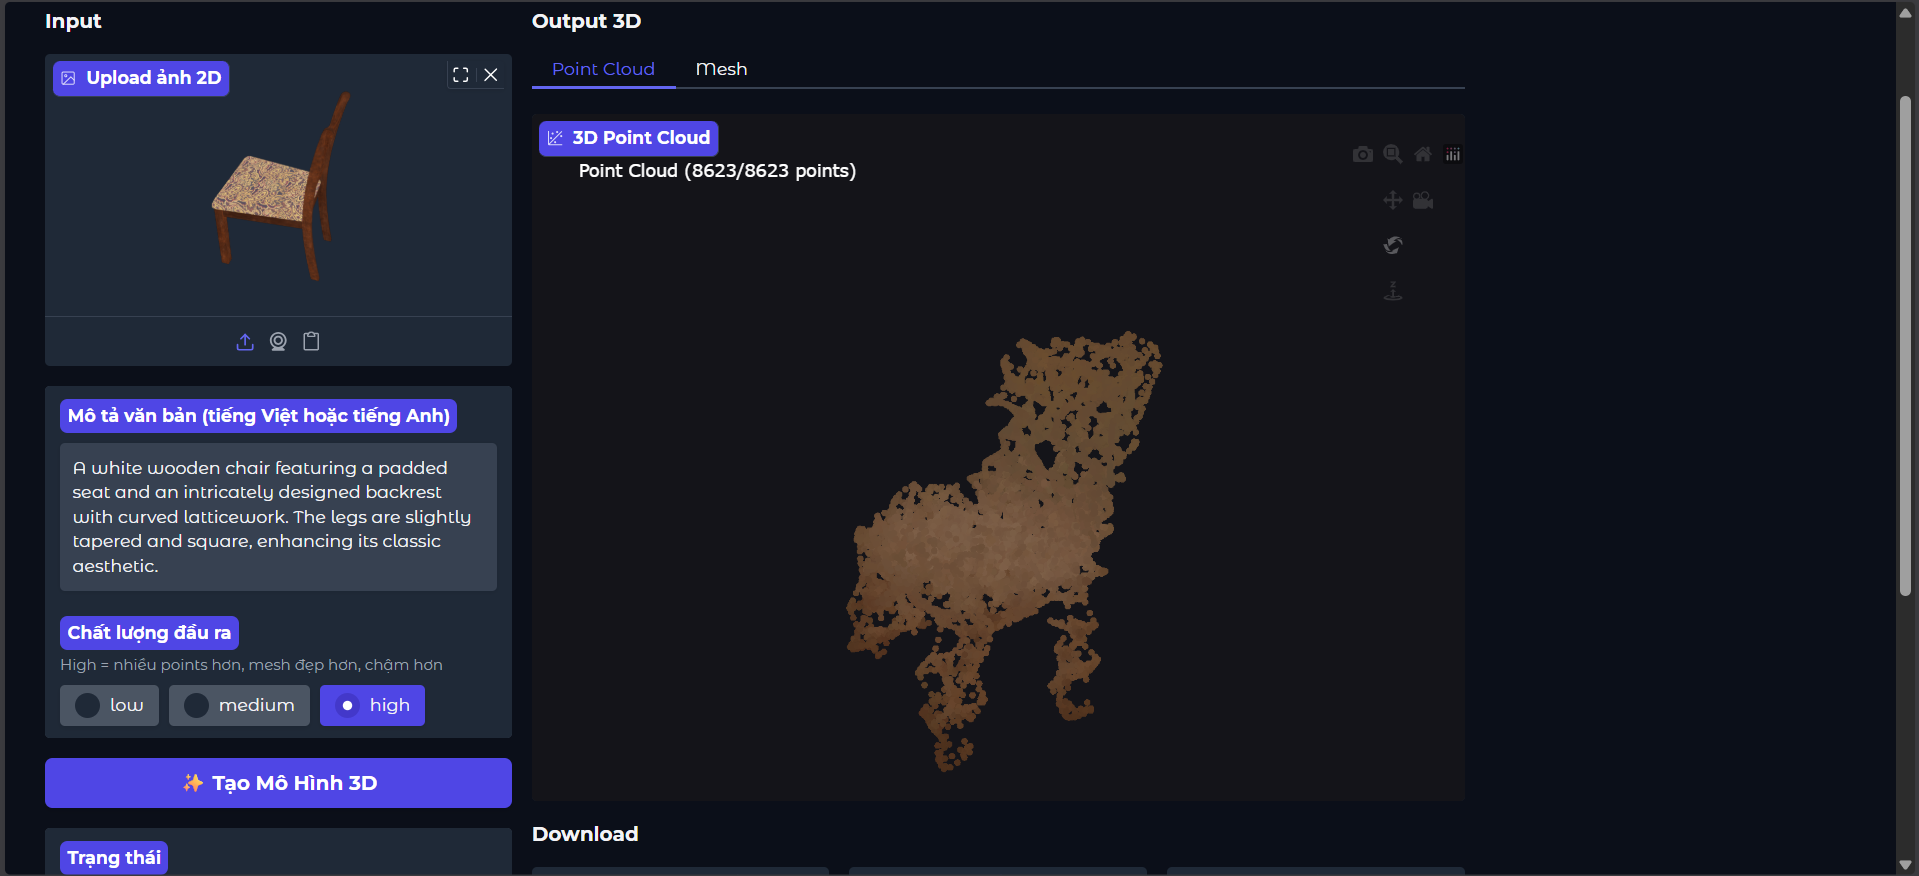
\includegraphics[width=0.9\linewidth]{image_report/result1_en.png}}
\caption{Kết quả sinh 3D với caption tiếng Anh.}
\label{fig:result_en}
\end{figure}

\begin{figure}[htbp]
\centerline{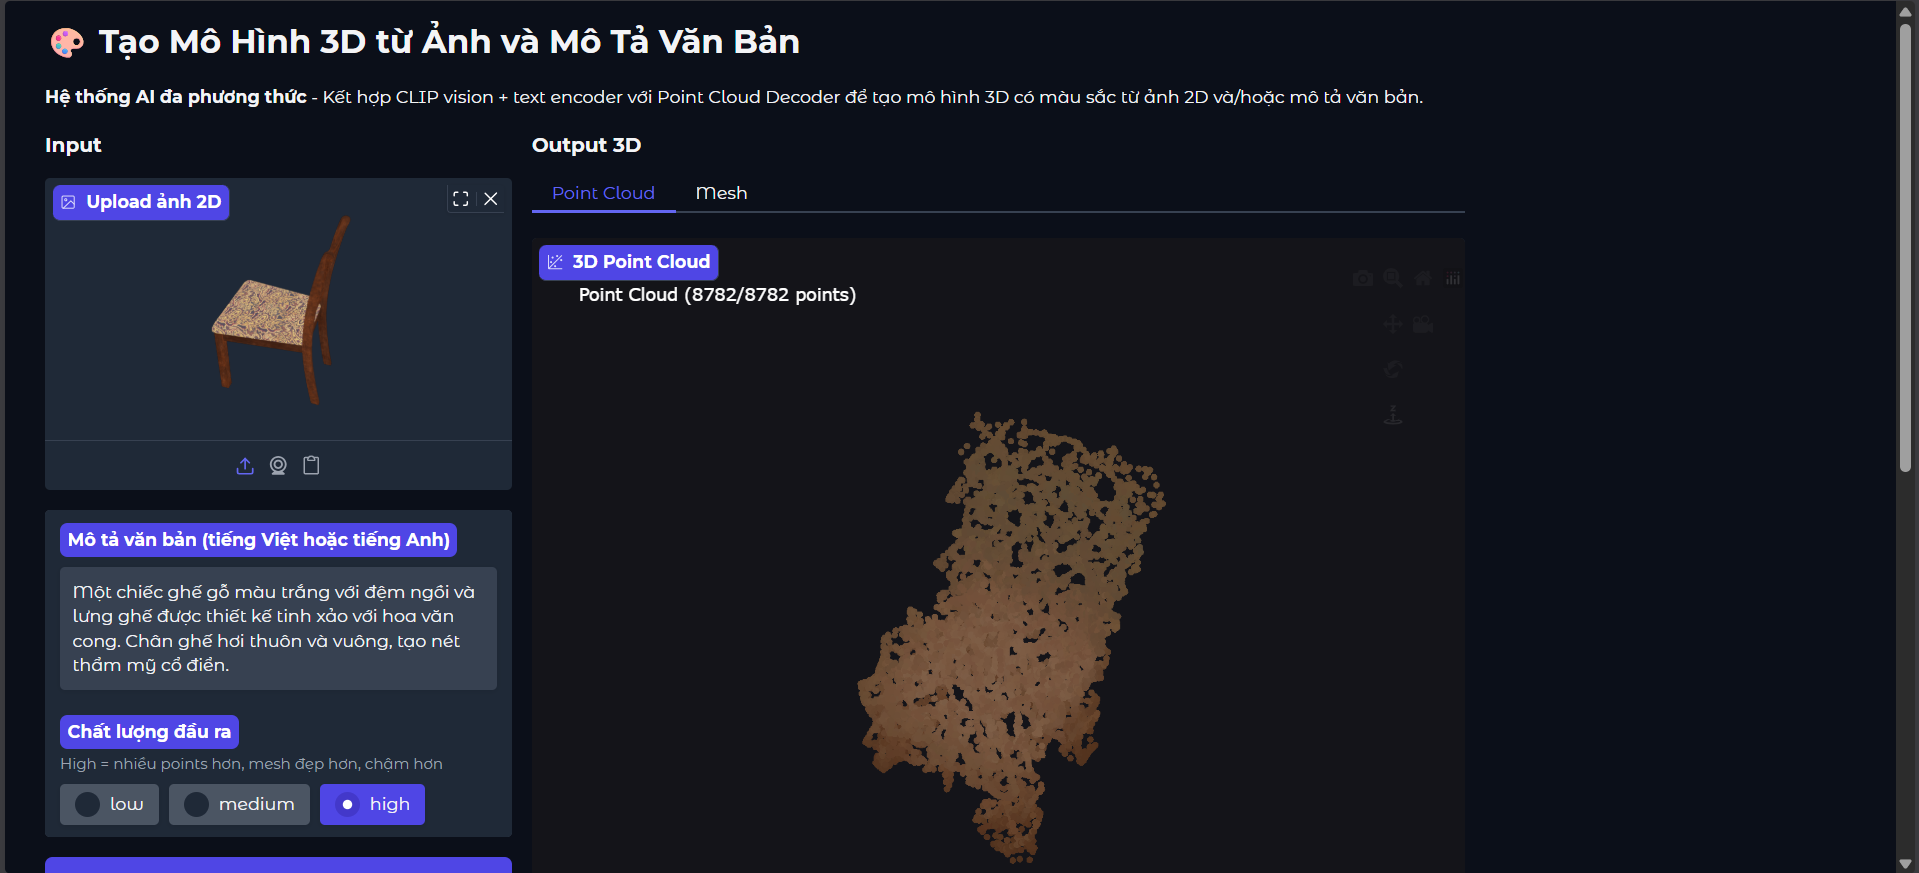
\includegraphics[width=0.9\linewidth]{image_report/result1_vi.png}}
\caption{Kết quả sinh 3D với caption tiếng Việt (tự động dịch sang tiếng Anh trước khi mã hóa).}
\label{fig:result_vi}
\end{figure}

% ─────────────────────────────────────────────
\section{Kết Luận}

Đồ án đã xây dựng thành công một hệ thống sinh đám mây điểm 3D đa phương thức kết hợp bộ mã hóa CLIP ViT-B/32 cố định với bộ giải mã Transformer theo chiến lược thô-đến-tinh. Mô hình được huấn luyện trên 11.464 đối tượng ABO trong 15 epoch trên GPU T4, đạt Chamfer Distance kiểm tra 0,0045 và F-Score@0.01 là 0,9592. Module dịch tự động tiếng Việt sang tiếng Anh giúp người dùng Việt Nam sử dụng hệ thống mà không làm giảm chất lượng đầu ra. Hướng phát triển tiếp theo bao gồm huấn luyện nhiều epoch hơn, tích hợp đầu vào đa góc nhìn và mở rộng sang các danh mục đối tượng ngoài ABO.

\section*{Lời Cảm Ơn}
Tác giả chân thành cảm ơn nền tảng Google Colab đã cung cấp tài nguyên GPU phục vụ quá trình huấn luyện mô hình trong đồ án này.

\begin{thebibliography}{00}

\bibitem{clip}
A. Radford et al., ``Learning transferable visual models from natural language supervision,''
in \textit{Proc. International Conference on Machine Learning (ICML)}, 2021, pp. 8748--8763.

\bibitem{cap3d}
T. Luo et al., ``Scalable 3D captioning with pretrained models,''
in \textit{Advances in Neural Information Processing Systems (NeurIPS)}, 2023.

\bibitem{marian}
J. Tiedemann and S. Thottingal, ``OPUS-MT -- building open translation services for the world,''
in \textit{Proc. European Association for Machine Translation (EAMT)}, 2020.

\end{thebibliography}

\end{document}
